%%%%%%%%%%%%%%%%%%%%%%%%%%%%%%%%%%%%%%%%%%%
\documentclass[12pt]{report}	%Doccument Class Specification

\setlength{\textwidth}{6.25in} % original 6.25 %Text Lenght SetUp
\setlength{\textheight}{8in}

\renewcommand{\baselinestretch}{1.3}	%Page Margin SetUp
\oddsidemargin 20pt    %  Left margin on odd-numbered pages.
\evensidemargin 20pt   %  Note that \oddsidemargin = \evensidemargin
\topmargin 0pt
\newcommand{\squeezeup}{\vspace{-0.6cm}}
%\renewcommand{\tableofcontents}{INDEX} 
\renewcommand*\contentsname{INDEX}
%%%%%%%%%%%%%%%%%%%%%%%%%%%%%%%%%%%%%%%%%%%

% Define Packages
\usepackage{amssymb}
\usepackage{amsmath}
\usepackage{subfigure}
\usepackage{algorithmic}
\usepackage{algorithm}
\usepackage{graphics}
\usepackage{epsfig}
\usepackage{listing}
\usepackage{graphicx}
\usepackage{titlesec}
\usepackage{url}
\usepackage{fancyhdr}
\usepackage{float}
\usepackage{fancybox}
\usepackage{xcolor}
\usepackage[left=3.81cm,top=2.54cm,right=2.54cm,bottom=3.175cm]{geometry}
\usepackage{pdfpages}
\usepackage[font=normalsize,labelfont=bf]{caption}
\usepackage[]{hyperref}
\usepackage[intoc]{nomencl}
%\renewcommand{\nomname}{List of %Abbreviations}
%\makenomenclature

\makeindex
%%%%%%%%%%%%%%%%%%%%%%%%%%%%%%%%%%%%%%%%%%%

%Change Font Size Of Titles
\titleformat{\chapter}[display]
  {\normalfont\large\bfseries\centering}{\chaptertitlename\ \thechapter}{14pt}{\large}
\titleformat{\section}{\normalsize \bfseries}{\thesection}{1em}{}
\titleformat{\subsection}{\normalsize \bfseries}{\thesubsection}{1em}{}
%%%%%%%%%%%%%%%%%%%%%%%%%%%%%%%%%%%%%%%%%%%

% Begin document "environment".

\begin{document} % Begin document "environment".

%%%%%%%%%%%%%%%%%%%%%%%%%%%%%%%%%%%%%%%%%%%	
%Title Page
	\begin{titlepage}   
		\thisfancypage{\setlength{\fboxsep}{10pt}\doublebox}{}
		\vspace*{0.1in}
		\begin{center}
%		{ \bf \small { [P-1]}}\\
		{ \bf { PRELIMENERY REPORT ON}}\\
		%{ \bf {REPORT ON}}\\
		\vspace{0.2in}
		{\Large \bf {``GRAY SCALE IMAGE COLORIZATION USING DEEP LEARNING''}}
		\\
		\vspace{0.2in}
		{\small  SUBMITTED TO THE SAVITRIBAI PHULE UNIVERSITY, PUNE \\ IN THE PARTIAL FULFILLMENT OF THE REQUIREMENTS \\ FOR THE AWARD OF THE DEGREE }\\
		{\bf OF}\\
		{\bf BACHELOR OF ENGINEERING (COMPUTER ENGINEERING)}\\
		\vspace{0.2in}
		{\bf SUBMITTED BY}\\
		\vspace{0.1in}
		{\small   Miss Divya Dinesh Pathak \hspace*{1.9 in} Exam No. 64 \\Miss Vaidehi Sudhir Patil \hspace*{1.9 in} Exam No. 35 \\Miss Gauri Pravin Sangale\hspace*{1.9 in} Exam No. 17 \\Miss Vranda Vikash Gupta\hspace*{1.9 in} Exam No. 29 }\\
		\vspace{0.1in}
		\begin{figure*}[h]
		\centerline{\psfig{figure=./IOIT logo.jpg,width=5in,height=1.25in}}
		\label{atcres}
		\end{figure*}
		{ \bf{ DEPARTMENT OF COMPUTER ENGINEERING}}\\ 
		\vspace{0.05in}
		{ \bf ALL INDIA SHRI SHIVAJI MEOMRIAL SOCIETY'S \\
		{\large \bf INSTITUTE OF INFORMATION TECHNOLOGY }}\\ 
		{\small KENNEDY ROAD, NEAR R.T.O. PUNE-411001 }\\ 
		\vspace{0.05in}	
%\begin{center} 
		{ \bf { SAVITRIBAI PULE PUNE UNIVERSITY}}\\	
		{ \bf \small { 2020-2021}}\\
	%	{ \bf \small { [p-2]}}\\	
			\end{center}
	\end{titlepage}
%%%%%%%%%%%%%%%%%%%%%%%%%%%%%%%%%%%%%%%%%%%
%Certificate
	\thisfancypage{\setlength{\fboxsep}{10pt}\doublebox}{}	
	
	\begin{titlepage} 
	
		\begin{center} 
\vspace{0.2in}
		\begin{figure*}[h]
				\centerline{\psfig{figure=./IOIT logo.jpg,width=5in,height=1.25in}}
%				\label{atcres}
\par\noindent\rule{\textwidth}{0.4pt}
			\end{figure*}
%\par\noindent\rule{\textwidth}{0.4pt}
		\end{center}
%	\begin{titlepage}
		\begin{center}
%		\begin{figure*}[h]
%		\centerline{\psfig{figure=./aissmsioitlogo.png,width=1.8in,height=1.4in}}
%		\label{atcres}
%		\end{figure*}
%		{\bf{ DEPARTMENT OF COMPUTER ENGINEERING}}\\
%		{ \bf All India Shri Shivaji Memorial Society's \\
%%		{\bf   PUNE 411041 }\\ 
		{\large\textbf{CERTIFICATE}}\\
%		\vspace{0.1in}
		{\small This is to certify that the project report entitles \\
			{\bf \large {``GRAY SCALE IMAGE COLORIZATION USING DEEP LEARNING''}}\\ Submitted by \\ 	
			{\small  Miss Divya Dinesh Pathak \hspace*{1.9 in} Exam No. 64 \\Miss Vaidehi Sudhir Patil \hspace*{1.9 in} Exam No. 35 \\Miss Gauri Pravin Sangale\hspace*{1.9 in} Exam No. 17  \\Miss Vranda Vikash Gupta\hspace*{1.9 in} Exam No. 29 }
		}
	\end{center}
			{
			is a bonafide student of this institute and the work has been carried out by him/her under the supervision of {\bf Dr. S.N. Zaware } and it is approved for the partial fulfillment of the requirement of Savitribai Phule Pune University, for the award of the degrees of {\bf Bachelor of Engineering} (Computer Engineering). }\\
		
		\vspace*{0.1in}
		\hspace*{0.4in} {\bf (Dr. S.N. Zaware) } \hspace*{1.6in}{\bf (Dr. S.N. Zaware)}\\
		\hspace*{1.1in}Guide \hspace*{2.7 in} Head\\
		\hspace*{0.2in}{Department of Computer Engineering} \hspace*{0.2 in}{Department of Computer Engineering}\\
		\vspace*{0.1in}\\
		\hspace*{2.3in} {\bf (Dr. P.B. Mane) }\\
		\hspace*{2.5 in} { Principal }\\
		\hspace*{0.9in}{AISSMS Institute of Information Technology, Pune-411001}\
		\vspace*{0.1in}\\
		\hspace*{0.4in}{Place: PUNE}\\
		\hspace*{0.4in}Date:
	\end{titlepage}
%%%%%%%%%%%%%%%%%%%%%%%%%%%%%%%%%%%%%%%%%%%

%%%%%%%%%%%%%%%%%%%%%%%%%%%%%%%%%%%%%%%%%%%

%%%%%%%%%%%%%%%%%%%%%%%%%%%%%%%%%%%%%%%%%%%

\pagenumbering{roman} %Roman PageNumbers

%%%%%%%%%%%%%%%%%%%%%%%%%%%%%%%%%%%%%%%%%%%


%Abstract
\addcontentsline{toc}{chapter}{Abstract}
\chapter*{ABSTRACT}

\hspace{2cm}Former approaches to the gray scale image colorization problem rely on manual methods with human intervention that produced some de-saturated results that are not likely to be true colorizations. Some of these methods were example based colorization, scribble based colorization. To fully automate the process of colorization, enormous amount of computation power and datasets are required which is daunting. So our project deals with colorization of gray scale human images. Our approach includes development of an autoencoder model for human face colorization. This can be useful to colorize old black and white movie snapshots, photos and documents. It is very difficult to deal with a general dataset due to limited memory and hardware specifications therefore the dataset of the proposed system is limited to human faces in RGB colour space.
\par{\hspace{0.5cm}} Among the various colorization techniques, convolutional neural network based colorization is selected because of its ability to deal with image datasets. Unlike the previous techniques, neural network based colorization method is a fully automatic technique which does not require any human assistance. This approach includes pre-processing, feature extraction, model generation and image post processing. The experimental results demonstrated that this method outperforms all the existing techniques. 

\section{Technical Keywords}

 {\bfseries Technical Key words related to our Proposed System are:}       
 \begin{itemize}
   \item 	CNN
   \item 	Encoder 
   \item 	Decoder
   \item	Google Colab
   \item	Image Colorization
   \item	Autoencoder
   \item    Mean squared error
 \end{itemize}
 \newpage
%%%%%%%%%%%%%%%%%%%%%%%%%%%%%%%%%%%%%%%%%%%

% Acknowledgement
\addcontentsline{toc}{chapter}{Acknowledgement}
\chapter*{ACKNOWLEDGMENT}
It gives us immense pleasure in presenting the preliminary project report on \\
 {\bf {``GRAY SCALE IMAGE COLORIZATION USING DEEP LEARNING''}} The success and the outcome of this report required a lot of guidance. We are very grateful to our guide \textbf{Dr. S.N. Zaware} who has provided expertise and encouragement. We thank madam who provided vision and knowledge that was very helpful throughout the research. All that we have done is only due to the great guidance. 


We would also like to extend our sincere thanks to Principal Dr.P.B. Mane, for his dynamic and valuable guidance throughout the project and providing the necessary facilities that helped us to complete our dissertation work.
%\ldots

\vspace{20mm} 
\begin{flushright}
{
\begin{minipage}{2.7 in}
\textbf{Miss Divya Dinesh Pathak}\\
\textbf{Miss Vaidehi Sudhir Patil}\\
\textbf{Miss Gauri Pravin Sangale}\\
\textbf{Miss Vranda Vikash Gupta}\\
% AISSMS IOIT, Pune.\\
\end{minipage}} \hfill
\end{flushright}
\newpage
%%%%%%%%%%%%%%%%%%%%%%%%%%%%%%%%%%%%%%%%%%%
%%%%%%%%%%%%%%%%%%%%%%%%%%%%%%%%%%%%%%%%%%%

%List Of Publications

%%%%%%%%%%%%%%%%%%%%%%%%%%%%%%%%%%%%%%%%%%%
\addcontentsline{toc}{chapter}{Index}
\tableofcontents
\newpage
%Default Pages
\newpage
%\addcontentsline{toc}{chapter}{List of Abbreviations}
%\printnomenclature
%\newpage
\addcontentsline{toc}{chapter}{List of Figures}
\listoffigures
\newpage	


%Default Pages - Table of Content

%%%%%%%%%%%%%%%%%%%%%%%%%%%%%%%%%%%%%%%%%%%

%Synopsis

%%%%%%%%%%%%%%%%%%%%%%%%%%%%%%%%%%%%%%%%%%%
%Technical Key Words

%%%%%%%%%%%%%%%%%%%%%%%%%%%%%%%%%%%%%%%%%%%


\pagenumbering{arabic}		%Page Numbering For Main Document

%%%%%%%%%%%%%%%%%%%%%%%%%%%%%%%%%%%%%%%%%%%

%Header And Footer
\fancyhf{}
\fancyhead[LE]{\leftmark}
\rhead[RO]{\scriptsize{\it GRAY SCALE IMAGE COLORIZATION USING DEEP LEARNING}}
\cfoot[LE,RO]{\thepage\\\scriptsize{Department of Computer Engineering, AISSMS's Institute of Information Technology, Pune. 2020-2021}}
\renewcommand{\footrulewidth}{0.4pt}
\pagestyle{fancy}
%%%%%%%%%%%%%%%%%%%%%%%%%%%%%%%%%%%%%%%%%%%

\chapter{INTRODUCTION}

\hspace{2cm}Image colorization is an interesting topic in image to - image translation. Nowadays, many cameras are still capturing grayscale images, like surveillance cameras and satellite cameras. In this project, we are going to implement image colorization framework based on deep learning methods. Our goal is to colorize old human photographs as these are found in plenty and need to be colorized at times. Our approach includes way to train the model using CNN(Convolution Neural Network). Training is done on RGB images and gray scale images. For training X image and Y image is considered where X is a gray scale image and Y is its corresponding RGB image. These images are then converted to .npy file which is a file containing images in vector form. Then the CNN autoencoder model is trained. This model is having conv2D layer which is used for storing the image as an encoded image. This model is saved and then use for further prediction. Finally testing is performed on gray scale images. These images would also be converted to .npy file and then conversion would take place. Mean squared error loss function is used to calculate the losses.
\par{\hspace{2cm}}Gray Scale image colorization is a very old research topic which mainly had focused on to reinstate the ancient images and documents. But scope of our project mainly concerns with colorization of human images since it is very difficult to deal with general dataset due to limited memory and hardware specifications.

\vspace{2 in}
\section{MOTIVATION}
The motivation behind choosing the domain is that gray Scale image colorization is a very old research topic which mainly had focused on different domains of colorization such as animals, landscape, etc. But there wasn’t any model that could colorize human faces accurately by following the method of conversion of images into .npy files. 


%\index{GSM} \nomenclature{GSM}{Global System for Mobiles} 

%\cite{6}.

\section{PROBLEM DEFINITION}
\begin{enumerate}
\item To automatically colorize gray scale human images using CNN without human intervention.
\item To use deep learning approach for image colorization.
\item To understand the accuracy of different cases based upon number of datasets used for training, epochs and batch size.
\item To calculate the losses using mean squared error function.
\end{enumerate}

\section{Input to the Project}
\subsection{Grayscale image (Passed as input X image)} 
\begin{itemize}

\item
Each pixel is represented using 8 bits which denotes the intensity of that pixel

\item
The higher the value, the greater the intensity. Current displays support 256 distinct shades of gray. Each one just a little bit lighter than the previous one.

\item
In the memory, a gray scale image is represented by a two dimensional array of bytes. Technically, this array is a ”channel”. So, a gray scale image has only one channel. And this channel represents the intensity of whites.

\end{itemize}

\subsection{RGB image (Passed as input Y image)} 
\begin{itemize}
\item
Corresponding RGB image of input grayscale image X is passed as input Y
\item
The model would then learn the comparative differences between theses X and Y images.

\end{itemize}

\subsection{Datasets}
The following are some sources for input images for training and testing purposes:
\begin{enumerate}
\item Kaggle
\item Wildfaces
\item Wikicrop
\end{enumerate}
\\

\begin{figure}[!h]
	\captionsetup{font=scriptsize}
	\begin{center}
		{\psfig{figure=./flower.jpg ,width=4.5in,height=4.5in}}
		%\centerline
		\caption{Gray Scale Image}
		\label{fig:1}
	\end{center}
	\squeezeup
\end{figure}
\newpage
%%%%%%%%%%%%%%%%%%%%%%%%%%%%%%%%%%%%%%%%%%%

\chapter{LITERATURE SURVEY}
\begin{enumerate}

	\item{\bf Title} : Fast Colorization of Grayscale Images by Convolutional Neural Network\\
	{\bf Author} : Titus, Swathy, and Jency Rena NM.\\
	{\bf Source} : International Conference on Circuits and Systems in Digital Enterprise Technology (ICCSDET). IEEE.\\
	{\bf Abstract} : This paper explores the fact that an image colorization problem can be fully automated using the Convolutional Neural Network. Here, they have used the CNN only for human faces due to resources and computation power constraints. They have trained the network on human RGB images. After successful training, this trained model is given to a neural network classifier. They have used ReLu activation function. \\

	\item{\bf Title} : Image Colorization with Convolutional Neural Networks\\
	{\bf Author} : An, Jiancheng\\
	{\bf Source} : International Congress on Image and Signal Processing, BioMedical Engineering and Informatics (CISP-BMEI). IEEE.\\
	{\bf Abstract} : The paper tries to solve the image colorization problem using a pre trained network VGG-16. VGG-16 is a CNN trained on datasets on ImageNet based on 1000 classes. The VGG-16 acts as a feature extractor and passes on the extracted features of the images to a CNN which predicts the color channels. They have trained the network on open source platform Caffe.\\
		
	\item{\bf Title} : Colorization using neural network ensemble.\\
	{\bf Author} : Cheng, Zezhou, Qingxiong Yang, and Bin Sheng.\\
	{\bf Source} : IEEE Transactions on Image Processing 26.11 (2017): 5491-5505.\\
	{\bf Abstract} : The paper discusses an approach that is a neural network ensemble. The paper claims that the existing neural network based image colorization systems uses thousands of similar images for training. When tested with an image which has not been trained on the network, colorization results are very poor. Hence, model ensemble neural network approach is dynamic and gives good colorized output images. \\
	
	\item{\bf Title} : Grayscale images colorization with convolutional neural networks\\
	{\bf Author} : An, Jiancheng, Koffi Gagnon Kpeyiton, and Qingnan Shi.\\
	{\bf Source} : Soft Computing 24.7 (2020): 4751-4758.\\
	{\bf Abstract} : The paper solves the image colorization problem using a pre trained network VGG-16. The RGB image is converted to LAB color space as it becomes easy to predict only two color channels ab rather than three (RGB). The model has been trained on open source platform Caffe. Cross entropy loss function has been used in the proposed system. \\
	
	\item{\bf Title} : Fully automatic image colorization based on Convolutional Neural Network\\
	{\bf Author} : Varga, Domonkos, and Tamás Szirányi.\\
	{\bf Source} : 2016 23rd International Conference on Pattern Recognition (ICPR). IEEE, 2016.\\
	{\bf Abstract} : The paper discusses various existing system that has been proposed till date for the image colorization problem. It has used VGG-16 pre trained network for the implementation. The network is trained on YUV color space. UV color space is predicted by the network. Various loss functions have been applied to measure the accuracy. \\

%%%%%%%%%%%%%%%%%%%%%%%%%%%%%%%%%%%%%%%%%%%%%%%%%%%

\end{enumerate}


\chapter{SOFTWARE REQUIREMENTS SPECIFICATION}

\section{Project Scope}
\begin{enumerate}
\item To automatically colorize gray scale images using CNN without human intervention. 
\item To apply deep learning in order to automate colorization process.
\item To effectively decide number of epochs and batch size so as to get good results.
\end{enumerate}


\section{System Requirements }
%\subsection{Database Requirements}
\subsection{Software Requirements}
\begin{enumerate}
	\item{\bf Keras :} Keras is an open-source software library that provides a Python interface for artificial neural networks.
	
	\item{\bf NumPy :} NumPy is a  Python library, used to support large, multi-dimensional arrays and vectors and large number of  mathematical functions to operate on these vectors.
	
	\item{\bf Tensorflow :} TensorFlow is a free and open-source software library for machine learning. It is used for deep neural networks and training.
	
    \item {\bf Google Colab :} Colab is a free open source online platform used for training deep neural networks.
    
    \item {\bf Scikit-image :} scikit-image is an  image processing Python library. It has algorithms for color space manipulation, like rgb2gray, for dimensional resizing, etc which is widely used in our project.
	
\end{enumerate}
\subsection{Hardware Requirements}
\begin{enumerate}
	\item{\bf Disk Space: } Minimum disk space of 500 GB is expected for computations and storage means.
	\item{\bf Processor} i5 CPU @1.60 GHz 1.80 GHz, 32-bit x32 OR 64-bit x64 processor is preferable.	
	\item{\bf Memory: } 4 GB RAM and above .
	\item{\bf GPU: } 2GB GPU and above.
\end{enumerate}
\section{System Implementation Plan}
In the system plan implementation the input is the GrayScale image. Using CNN the image is colorized. The expected output is the colorized image.
\begin{figure}[!h]
	\captionsetup{font=scriptsize}
	\begin{center}
		{\psfig{figure=./plan.PNG,width=5.5in,height=6.5in}}
		%\centerline
		\caption{System Plan}
		\label{fig:2}
	\end{center}
	\squeezeup
\end{figure}

%%%%%%%%%%%%%%%%%%%%%%%%%%%%%%%%%%%%%%%%%%%%%%%%%%%%%%%%%%%%%
\chapter{SYSTEM DESIGN}

\section{System Architecture}
\section{System Architecture}
\begin{enumerate}
\item Input Gray scale image
\item Auto-encoder network
\item Image post-processing
\item Output is the colorized image
\end{enumerate}
\begin{figure}[!h]
	\captionsetup{font=scriptsize}
	\begin{center}
		{\psfig{figure=./Revised system architecture diag.PNG,width=5.5in,height=6.5in}}
		%\centerline
		\caption{System Architecture}
		\label{fig:3}
	\end{center}
	\squeezeup
\end{figure}
\newpage

\section{UML Diagrams}
\subsection{Activity Diagram}
\begin{itemize}
	\item	Activity Diagram is a behavioral diagram presenting the actors their functions performed.
	\item	They also include the swim lanes and the forks and joins.
	\item	The represent the individual  lane as their entire activities and the functionality carried out by that particular actor in the respective lanes.
	\item	Input is being provided by the user and the output is being given back to the user.
	
\end{itemize}
\begin{figure}[!t]
	\captionsetup{font=scriptsize}
	\begin{center}
		{\psfig{figure=./Revised activity diagram.PNG,width=3.0in,height=6.8in}}
		%\centerline
		\caption{Activity Diagram}
		\label{fig:5}
	\end{center}
	\squeezeup
\end{figure}
\newpage

\subsection{Use case Diagram}
Use Case diagram is used for representing the problem statement that is the actors in it, their functionality in an behavioral manner. They are useful when the system is to be in the programmatic execution.
\begin{figure}[!h]
	\captionsetup{font=scriptsize}
	\begin{center}
		{\psfig{figure=./UseCase.png,width=6.5in,height=7.0in}}
		%\centerline
	\caption{Use Case Diagram}
		\label{fig:6}
	\end{center}
	\squeezeup
\end{figure}
\newpage
\begin{itemize}
	\item Use Case diagram has the actors and all the functional blocks.
	\item{\bf Actors}
	\begin{enumerate}
		\item User
		\item Colorization System
	\end{enumerate}
	\item Functional Blocks include the stepwise execution of the entire system that is the form of different procedures (functionality).
	\item	Input to the every function in this diagram is the output from the previous state.
	\newpage
\end{itemize}

\section{Data Flow Diagrams}

\subsection{DFD Level 0}
	\begin{figure}[!h]
		\captionsetup{font=scriptsize}
		\begin{center}
			{\psfig{figure=./DFD-0.PNG,width=6.5in,height=1.5in}}
			%\centerline
			\caption{DFD Level 0}
			\label{fig:7}
		\end{center}
		\squeezeup
	\end{figure}
	 In the data dependency diagram at level zero the input is the gray scale dataset and the output is the colorized image.

\subsection{DFD Level 1}
	\begin{figure}[!h]
		\captionsetup{font=scriptsize}
		\begin{center}
			{\psfig{figure=./level-1.PNG,width=6.5in,height=1.5in}}
			%\centerline
			\caption{DFD Level 1}
			\label{fig:7}
		\end{center}
		\squeezeup
	\end{figure}
	 In the data dependency diagram at level one the input is the gray scale dataset and the output is the RGB image. 
	\subsection{DFD Level 2}
	\begin{figure}[!h]
		\captionsetup{font=scriptsize}
		\begin{center}
			{\psfig{figure=./level-2.PNG,width=5.5in,height=5.5in}}
			%\centerline
			\caption{DFD Level 2}
			\label{fig:8}
		\end{center}
		\squeezeup
	\end{figure}
In the data dependency diagram at level two the input is the gray scale dataset and colorized image and the output is the colorized image. The input image is fed to the CNN model.

%%%%%%%%%%%%%%%%%%%%%%%%%%%%%%%%%%%%%%%%%%%%%%%%%%%%%
\chapter{LIST OF MODULES AND FUNCTIONALITY}


\begin{itemize}


\item
{\bfseries Input Gray scale image pre-processing:}

			\begin{enumerate}
			
			    \item	
	                Perform dimension scaling of the input image based on the Dataset used for training.

				\item
					{\bfseries For train images }: Train Images include RGB as well as gray scale images. These images are converted to .npy file. .npy file is a file containing images in vector form. The advantage of using .npy file is that they are convenient in terms of loading, pre-processing and training the model.
				\item
					{\bfseries For test images }: These are gray scale images. Even these images need to be converted to .npy file.

\end{enumerate}
	

\item{\bfseries Train the CNN auto-encoder model : } 
\begin{enumerate}

	\item
	Model is having conv2D layer to minimize image to store it as an encoded image. These conv2D layers act as encoder.
	\item
	After passing through the encoder the input image is converted to an intermediate image ‘Z’. This ‘Z’ image then acts as an input to the decoder.
	\item
	Conv2D transpose layer generates colorized image from the encoded representation. These conv2D transpose layers act as decoder.
	\item
	Perform training of data using google colab.

\end{enumerate}

\item
{\bfseries Save the trained model :} The CNN model thus formed for colorizing human images must then be saved for prediction purpose.

\item
{\bfseries Perform prediction on the trained file :} The saved trained model can now be used to perform predictions for conversion of images.

\item
{\bfseries Calculate losses using mean squared error loss function :} The loss is the mean overseen data of the squared differences between true and predicted values, or writing it as a formula.

{\bfseries Image post processing :} The .npy files are converted back to RGB image which is the output image. Image denormalization is performed on these images.

{\bfseries Comparative study of accuracy over several epochs and batch size :} Training is carried out over different epochs and batch size in order to understand the difference and relation between them.

\end{itemize}

%%%%%%%%%%%%%%%%%%%%%%%%%%%%%%%%%%%%%%%%%%%%%%%%%%%%%%%%%%%%%%%%%%%%%%%%%%%%%%%%%%%%%%%%%%%%%%%%%%%%%%%%5

\chapter{ALGORITHM}
{\bfseries Convolutional Neural Network :}We will be using Convolutional Neural Network (CNN) architecture which is a specialized type of neural network model designed for working with two-dimensional image data. The processed input image is first passed to the pooling layer which goes through various convolutional layers after pooling. CNN architecture consists of various convolutional layers which apply various filters to the image on which pooling is performed. The Fully Connected layer classifies images into labels, which follows a stack of Conv. layers. The final layer is the softmax layer which is used as the activation function.

%%%%%%%%%%%%%%%%%%%%%%%%%%%%%%%%%%%%%%%%%%%%%%%%%%%%%%%%%%%%%%%%%%%%%%%%%%%%%%%%%%%%%%%%%%%%%%%%%%%%%%%%5

\chapter{RELEVANT MATHEMATICS ASSOCIATED}

\label{sec:math}
SYSTEM DESCRIPTION:
\begin{itemize} 
\item {\bfseries Input :} Gray Scale Image	 
\item {\bfseries Output :} Colorized image
 
\item {\bfseries Functions :}

    

    {\bfseries Loss Functions :} 
    We will be using following loss function in our project.\\ 
    {\bfseries Mean squared error -} The goal is to minimize the loss over the training set. In the image colorization,the training datasets consists of thousands of color images as Y and their grayscale versions as X. The loss is the mean overseen data of the squared differences between true and predicted values.\\
    \begin{center}
            $MSE = \sum_{n=1}^{n} (y_i-y_i^p)^{2} $	
    \end{center}
	
\end{itemize}
%%%%%%%%%%%%%%%%%%%%%%%%%%%%%%%%%%%%
\chapter{OTHER SPECIFICATION}
\section{Advantages}
\begin{itemize}
	\item Colorization results are very accurate for the images containing human figures.

\end{itemize}
\section{Limitations}
\begin{itemize}
	\item The system requires a very large dataset for training and hence, lot of computation power and time.
	
	
\end{itemize}
\section{Applications}
\begin{enumerate}
	\item Can be used for colorization of Black and White old flims
	\item Can be used to reinstate old documents
        \item Can be used for colorization of survellience images, MRI images and satellite images.
	
\end{enumerate}

%%%%%%%%%%%%%%%%%%%%%%%%%%%%%%%%%%%%%%%%%%%%
\chapter{CONCLUSIONS AND FUTURE WORK}
\section{Conclusion}
Grayscale Images are successfully colorized using CNN autoencoder model and accuracy is evaulated in accordance with the number of datasets used for training, epochs and batch size.


\section{Future work}
\begin{enumerate}
	\item	Use different color spaces. 
        \item Train the model for images of variable size/type.
        \item Reduce the size of quantized bins.
	
\end{enumerate}

\newpage
\section{Output}
Output will be predicted colorized image.
\begin{center}

\begin{figure}[htp]

\centering
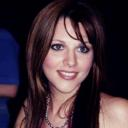
\includegraphics[width=.3\textwidth]{./GroundTruth.jpg}
\caption{Ground Truth}
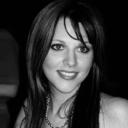
\includegraphics[width=.3\textwidth]{./Input.jpg}
\caption{Input}
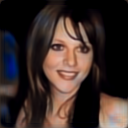
\includegraphics[width=.3\textwidth]{./Predicted.png}
\caption{Predicted}

\label{fig:figure3}

\end{figure}

\end{center}

\addcontentsline{toc}{chapter}{Appendix A}
\chapter*{ANNEXURE A}
\label{Appendix A}
\begin{center}
    \Large {\bfseries Declaration}
\end{center}
We hereby declare that the project work entitled “Gray Scale Image Colorization using Deep Learning” submitted to the Savitribai Phule Pune University, is our original work under the guidance of Dr. S. N. Zaware, Head of Department Computer Engineering, AISSMS IOIT. This project work is submitted in the partial fulfilment of the requirements for the award of the degree of Bachelors in Computer Engineering. The results evaluated in this report have not been submitted to any other University or Institute for the award of any degree or diploma.

\vspace{0.5in}
{\small\hspace*{3.3 in} Miss Divya Dinesh Pathak\\ \hspace*{3.5 in} Miss Vaidehi Sudhir Patil\\ \hspace*{3.5 in} Miss Gauri Pravin Sangale\\ \hspace*{3.5 in}  Miss Vranda Vikash Gupta\\}


\addcontentsline{toc}{chapter}{Appendix B}
\chapter*{ANNEXURE B: PLAGIARISM}
\label{Appendix B}



%\includepdf[scale=0.9, pages={1-4}]{xml.pdf}
\newpage
%%%%%%%%%%%%%%%%%%%%%%%%%%%%%%%%%%%%%%%%%%%

%Bibliography
\addcontentsline{toc}{chapter}{Bibliography}
%\renewcommand{\headrulewidth}{0pt}
%\fancyhf{}
\begin{thebibliography}{99}

\bibitem{1}
An, Jiancheng, Koffi Gagnon Kpeyiton, and Qingnan Shi."Grayscale images colorization with convolutional neural networks." Soft Computing 24.7 (2020): 4751-4758.

\bibitem{2}
 Kiani, Leila, Masoud Saeed, and Hossein Nezamabadi-pour. "Image Colorization Using Generative Adversarial Networks and Transfer Learning." 2020 International Conference on Machine Vision and Image Processing (MVIP). IEEE, 2020.

\bibitem{3}
Sindhuja Kotala;  Srividya Tirumalasetti; Vudaru Nemitha; Swapna Munigala.“Automatic Colorization of Black and White Images using Deep Learning”

\bibitem{4}
Górriz, Marc, et al. "End-to-End Conditional GAN-based Architectures for Image Colourisation." arXiv preprint arXiv:1908.09873 (2019).

\bibitem{5}
Dabas, Chetna, et al. "Implementation of image colorization with convolutional neural network." International Journal of System Assurance Engineering and Management (2020): 1-10.

\bibitem{6}
Zhang, Richard, Phillip Isola, and Alexei A. Efros. "Colorful image colorization." European conference on computer vision. Springer, Cham, 2016.

\bibitem{7}
Hwang, Jeff, and You Zhou. "Image colorization with deep convolutional neural networks." Stanford University, Tech. Rep.. 2016.

\bibitem{8}
Fu, Qiwen, Wei-Ting Hsu, and Mu-Heng Yang. "Colorization Using ConvNet and GAN." Stanford University. 2017. 1-8.

\end{thebibliography}

\newpage
%%%%%%%%%%%%%%%%%%%%%%%%%%%%%%%%%%%%%%%%%%%

\end{document}

